\section{Grundlagen}
\label{cha:grundlagen}
%Im Grundlagenkapitel stellen Sie das Basiswissen für die weiteren Kapitel vor.
%Hierzu können neben theoretischen Konzepten auch die historische Entwicklung
%und aktuelle Forschungsvorhaben gehören. Idealerweise bedient man sich hier
%mehrerer verschiedener Quellen, um die Ausführungen zu belegen.

%Nachfolgend werden einige Formalitäten der Arbeit dargestellt.
In dieser Arbeit soll ein Vorgehensmodell für Migrationen herkömmlicher 
Software in die Cloud entwickelt werden, das sich an unabhängige 
Softwarehersteller richtet. Aus diesem Ziel ergeben sich grundlegende Fragen, 
die in diesem Kapitel beantwortet werden sollen:
\begin{itemize}
	\item Welche Vorteile bietet die Cloud, welche Nachteile sind mit ihr verbunden und wie lassen sie sich
erzielen beziehungsweise vermeiden? 
	\item Inwiefern unterscheiden sich Cloud-Migrationen von herkömmlichen
Migrationen in der IT und wie lassen sie sich zum Outsourcing abgrenzen? 
	\item Was wird in dieser Arbeit unter unabhängigen 
Softwareherstellern ("`Independent Software Vendors"' -- ISV)  
verstanden? Welche Besonderheiten weisen sie und ihre Projekte auf und welchen
Einfluss haben diese Besonderheiten auf Cloud-Migrationen?
	\item Welche Faktoren beeinflussen die Cloud-Migration und ihren
Erfolg?
\end{itemize}
Dieses Kapitel wird von der Vorstellung des Fünf-Phasen-Modells abgeschlossen,
auf dem das entwickelte Vorgehensmodell basiert. Auch wird die Wahl für dieses
Modell als Arbeitsgrundlage begründet.

\subsection{Migration und Cloud-Migration}
\label{cha:definition_cloud-migration}

Die Migration von Software, wird in der Norm ISO/IEC 14764 "`Software
Engineering -- Software Life Cycle Processes -- Maintenance"' als spezielle
Form der Wartung, nämlich als anpassende Wartung ("`Adaptive Maintenance"') und
Weiterentwicklung definiert, bei der eine Software nach Auslieferung geändert
wird, um das Produkt in geänderten oder sich ändernden Umgebungen nutzbar zu
halten \pcite{}{}{characterizing_software_architecture_changes}. \\
Beispiel für eine solche Migration ist der Umzug einer Software auf neue
Hardware mit aktualisiertem Betriebssystem. Grund für den Umzug könnte ein
technischer sein, wie etwa dass keine Ersatzteile mehr für die vorhandene
Hardware angeboten werden oder dass der Support des Herstellers für das laufende
Betriebssystem ausläuft. Aber auch wirtschaftliche Gründe, wie etwa eine
geforderte, höhere Leistungsfähigkeit oder ein geringerer Energieverbrauch des
neuen Systems sind denkbar. \\
Um die Software weiter zu betreiben, muss sie gegebenenfalls an das
aktualisierte Betriebssystem oder die Laufzeitumgebung angepasst werden.
Je standardisierter und verbreiteter die Anforderung der zu migrierenden
Software, desto geringer werden die nötigen Anpassungen an der
Software ausfallen, womit die Migration einfacher und kostengünstiger wird.
Eventuell wird lediglich eine virtuelle Maschine auf einem neuen Server
gestartet. 

Eine solche virtuelle Maschine ließe sich auch in der Cloud starten. Auf diese 
Weise ließen sich jedoch nicht die folgenden Vorteile realisieren, die 
\citeflow{exploring_the_factors} als Hauptgründe für eine Migration in die 
Cloud identifiziert haben:
\begin{description}
	\item[Kosteneinsparungen] Cloud-Anbieter, die große Rechenzentren
mit vielen Servern betreiben, können die Total Cost of Ownership pro Server um
bis zu 80\% reduzieren (Vgl. Abbildung~\ref{fig:tco_reduction}).

\begin{figure}[!h]
\begin{center}
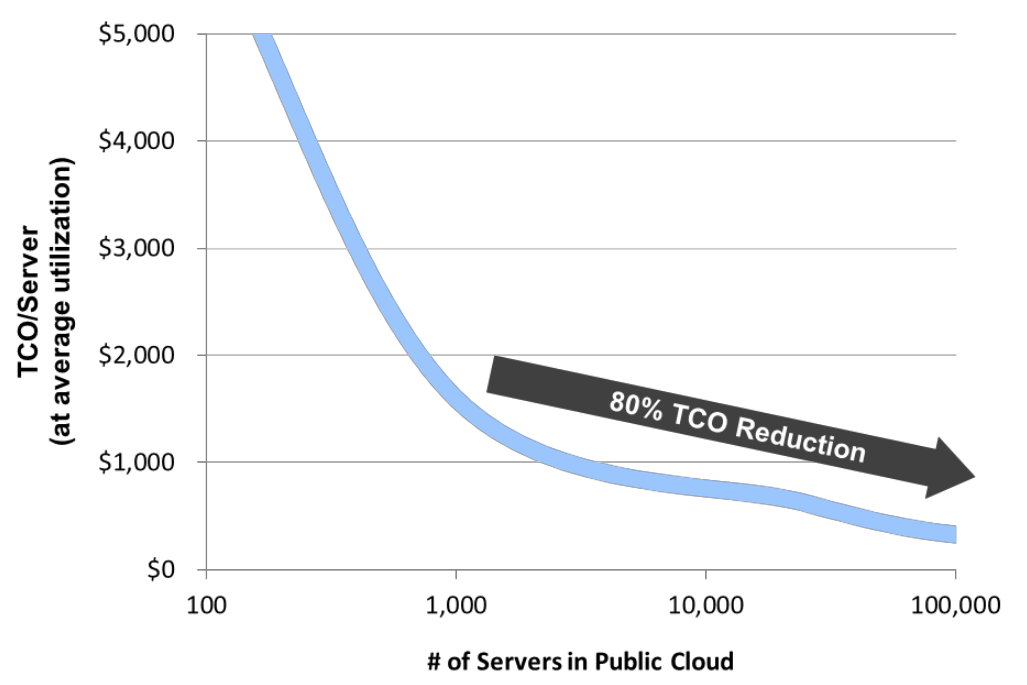
\includegraphics[width=0.8\textwidth]{images/tco_reduction.png}
\caption{Total Cost of Ownership/Server
aus \protect\citeflow{economics_of_the_cloud}}
\label{fig:tco_reduction}
\end{center}
\end{figure}
 Hauptsächlich geschieht dies über die Faktoren Energie-, Lohn- und
Hardwarekosten. Energiekosten lassen sich durch die Wahl eines Standortes
mit günstigem Strom und niedrigen Umgebungstemperaturen senken. Durch
Automatisierungstechniken lassen sich die Zahl der Server, die ein Administrator
betreibt, verzehnfachen, wodurch die Lohnkosten sinken. Hardwarekosten fallen
durch bessere Verhandlungspositionen großer Cloud-Anbieter niedriger aus 
\pcite{}{}{cloud_migration}.

Die niedrigeren Kosten werden über den Markt teilweise an die Kunden weitergegeben. Diese
können die kapitalintensive Beschaffung der Hard- und Software sowie die
Vorhaltung eigener Personalressourcen zur Entwicklung und Wartung reduzieren \pcite{}{}{Repschlaeger2010}.

	\item[Effiziente Ressourcennutzung] In der konventionellen IT-Welt
werden geschätzte 80\% der Ressourcen dazu verwendet, bestehende Infrastruktur
und Dienstleistungen zu betreiben. Dadurch bleibt wenig Kapazität für wertstiftende
Tätigkeiten, wie die Entwicklung neuer Geschäftsfelder oder die Umsetzung von
Kundenwünschen. Cloud-Nutzung kann
dieses Verhältnis der Innovation verschieben \pcite{}{}{economics_of_the_cloud}.

	\item[Automatisierte, schnelle und unbegrenzte Skalierbarkeit der
Ressourcen] Die Zuteilung zusätzlicher, auf den Kunden unbegrenzt wirkender
Rechenleistung, erfolgt in der Cloud entweder über ein einfaches Webformular oder,
ausgerichtet am momentanen Bedarf, voll automatisch. Da der Kunde nur das
bezahlen muss, was er benötigt, ist die Cloud gerade für Start-ups, kleine und
mittlere Unternehmen interessant. Aber auch für Unternehmen, die entweder einen stark
schwankenden oder nicht abschätzbaren Bedarf haben. Die Gefahr zu viel
Rechenleistung vorzuhalten, was zu unnötig hohen Kosten führt oder zu wenig
Rechenleistung, was Kunden abschrecken könnte,
sinkt 
\pcite{}{}{
economics_of_the_cloud, a_holistic_model_for_making_cloud_migration_decision,
migrating_to_the_cloud_lessons_and_limitations}.

Das schnelle Deployment in der Cloud ermöglicht es, neue Ideen sehr
schnell zu implementieren, zu testen (falls gewünscht sogar im Vergleich zu
anderen Lösungen) und auszuwerten. Dadurch kann die Innovationsgeschwindigkeit,
Flexibilität und die "`Time to Market"' beachtlich gesteigert werden 
\pcite{}{}{factors_in_development_and_adoption,
decision-making_in_cloud_computing_environments, cloud_migration}.

	\item[Geringerer Wartungsaufwand] Die Cloud treibt die Standardisierung
von Schnittstellen voran, sodass bestehende Funktionalitäten leichter
wiederverwendet werden können. Dadurch wird die Weiterentwicklung und Wartung
von Software reduziert \pcite{}{}{economics_of_the_cloud}.
\end{description}

\begin{comment}
Um von diesen Vorteilen profitieren zu können müssen 
die Software selbst, sowie Arbeitsprozesse und Geschäftsmodell angepasst 
werden. Da Umfang der Änderungen nicht mehr unter die oben genannte 
"`Weiterentwicklung"' fällt, wird von Cloud-Migrationen als Abgrenzung zu 
herkömmlichen Migrationen gesprochen. 
\pcite{}{}{framework_for_architecture-driven_migration}
\end{comment}


Der Grad, in dem diese Vorteile realisiert werden, hängt davon ab, 
in welchem Umfang Leistungen in der Cloud in Anspruch genommen werden, was 
wiederum Einfluss auf den Migrationsprozess hat \pcite{}{213}{Pahl2013}. Zur 
Kategorisierung des Leistungsumfangs dienen "`as a Service"'-Modelle. Es
gibt viele dieser Modelle - \citeflow{xAsAService} zählt 35
Varianten - die mehr oder weniger verbreitet sind und mit "`Everything as a
Service"', abgekürzt als EaaS oder XaaS zusammengefasst werden. Dabei werden
nicht nur Technologien als Dienstleistung angeboten, sondern auch Ziele; so gibt
es beispielsweise auch "`Hardware-as-a-Service (HaaS)"' und
"`Business-Process-as-a-Service (BPaaS)"'
\pcite{}{}{emerging_paradigms_and_areas_for_expansion, benlian_saas_2010}.
\begin{figure}%[h]
\begin{center}
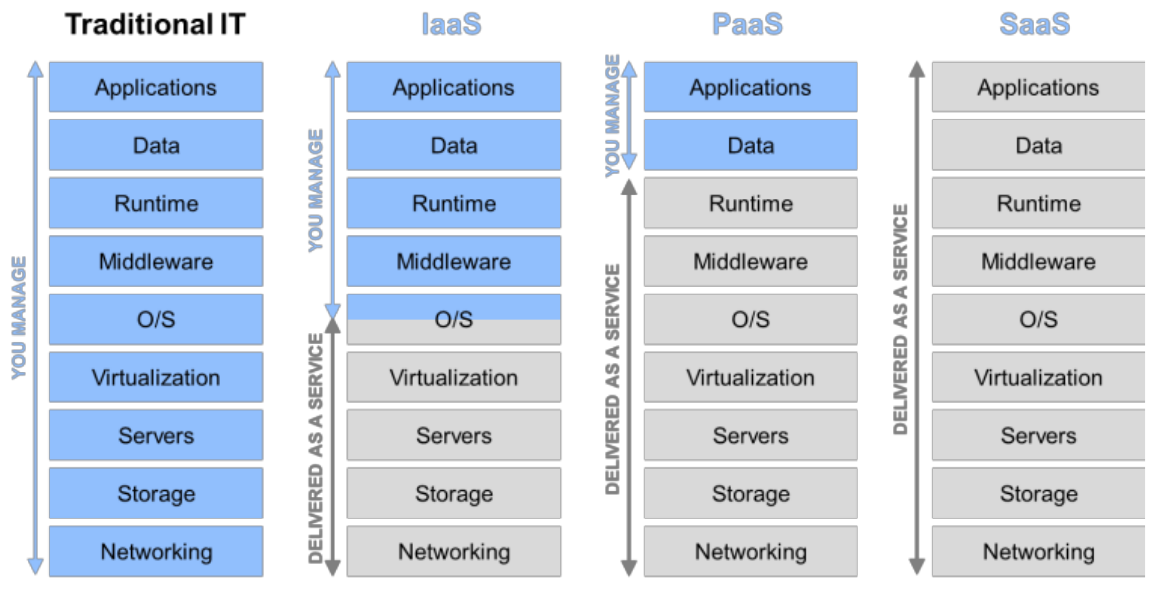
\includegraphics[width=\textwidth]{images/XaaS_im_Vergleich.png}
\caption{XaaS im Vergleich: Umfang von
Dienstleistung und Eigenverantwortung. Aus
\protect\citeflow{economics_of_the_cloud} }
\label{fig:xaas_im_vergleich}
\end{center}
\end{figure}

Anerkannt sind die vom amerikanischen "`National Institute of Standards and Technology (NIST)"' definierten Service Modelle, die sich im Anteil der selbst zu verwaltenden, technologischen Anteile (Integrationstiefe)
unterscheiden und in dieser Hinsicht in Abbildung~\ref{fig:xaas_im_vergleich}
mit der herkömmlichen IT verglichen werden \pcite{}{}{NIST,thoughtsOnCloud,softwareindustrie2015}:
\begin{description}
	\item[Infrastructure as a Service (IaaS)] Dem Kunden werden Netzwerk,
Speicher und Rechenleistung zur Verfügung gestellt. Über die darauf laufende
Software, teilweise sogar über das Betriebssystem, kann der Kunde selbst verfügen. \\
Kunden versprechen sich von IaaS vor allem Flexibilität in der Bereitstellung
und dem Betrieb von Servern, Datenspeichern und Netzwerkressourcen \pcite{}{213}{Pahl2013}.
	\item[Platform as a Service (PaaS)] Der Kunde kann bereitgestellte
oder selbst entwickelte Software in der Cloud laufen lassen und eventuell
Einfluss auf die Anwendungsumgebung nehmen. 
	\item[Software as a Service (SaaS)] Der Kunde kann eine vom Anbieter
bereitgestellte Software nutzen und in begrenztem Maße konfigurieren.
\end{description}

Das für die Migration genannte Beispiel, eine virtuelle Maschine zu
verschieben, lässt sich mit Abbildung~\ref{fig:xaas_im_vergleich} für den
Cloud-Fall dem Modell IaaS zuordnen. Der Cloud-Kunde muss sich in diesem Fall,
neben der eigentlichen Anwendung nach wie vor um das virtualisierte
Betriebssystem, Middleware, Laufzeitumgebung und Datenhaltung kümmern. Um die
Vorteile der Cloud besser auszuschöpfen, müsste die Anwendung entweder so
angepasst werden, dass sie auf einer zur Verfügung gestellten, fremdverwalteten
Laufzeitumgebung läuft (PaaS). Oder es wird eine bestehende Anwendung in der
Cloud genutzt und gegebenenfalls angepasst (SaaS). Beide Optimierungen
machen das Treffen konsequenzenreicher, kritischer Entscheidungen nötig, die 
nicht nur technische, sondern auch betriebswirtschaftliche und 
strategische Aspekte betreffen \pcite{}{}{migration_to_paas_clouds}.
Aus diesem Grund ist eine Cloud-Migration\footnote{Der Vollständigkeit halber
hier eine formale Definition der Cloud-Migration: "`Prozess der anteiligen
oder
vollständigen Bereitstellung von digitalen Gütern, Dienstleistungen,
IT-Ressourcen oder Anwendungen in der Cloud"'}
\pcite{}{}{Pahl2013} in ihrem Umfang viel mehr als eine Weiterentwicklung 
herkömmlicher Migrationen und erfordert eine dementsprechende, viel 
umfangreichere
Planung \pcite{}{}{framework_for_architecture-driven_migration,
a_review_of_the_current_level_of_support_to_aid_decisions_for_migrating}.

Für die zu migrierende Software gibt es zahlreiche Namen, zum Beispiel 
"`Software as a Product"' (SaaP) 
\pcite{}{}{changes_in_requirements_engineering}, "`Software as a Good"' 
\pcite{}{}{transitioning_to_saas} oder "`Legacy System"' 
\pcite{}{}{framework_for_architecture-driven_migration}. In dieser Arbeit wird 
der Begriff "`On-Premise-Software"' verwendet.

Der Ablauf von Cloud-Migrationen lässt sich in die folgenden Kategorien 
unterteilen \citeflow{exploring_the_factors}: 
\begin{description}
	\item[Ersetzen] Einzelne Komponenten einer bestehenden Anwendung werden
durch Dienste in der Cloud ersetzt. Andere Komponenten, die mit diesen
ersetzten Komponenten interagieren, werden umkonfiguriert. Buzzwörter zu dieser 
Kategorie sind "`Service Oriented Architecture"' (SOA) und "`Microservices"': 
Anstatt Anwendungen als Monolithen gewaltigen Umfangs zu entwerfen, werden sie 
aus kleinere, wiederverwertbaren Diensten konstruiert, die über Schnittstellen 
verbunden werden.
	\item[Partielle Migration] Anstatt Komponenten komplett durch Cloud-Dienste zu
ersetzen, werden sie in die Cloud migriert.
	\item[Migration der ganzen Anwendung] Diesem Typus entspricht das 
Beispiel von oben: Eine Anwendung wird in ihrer virtuellen Maschine in die 
Cloud umgezogen.
	\item[Cloudify] Die Anwendung wird in Gänze an die Cloud und ihre
Charakteristika angepasst und mit Cloud-Diensten neu entwickelt. Dieser Maxime 
folgt das in dieser Arbeit vorgestellte Modell.
\end{description}

%\subsubsection{Abgrenzung zum Outsourcing}

\subsection{Softwarehersteller: Independent Software Vendor (ISV)}
\label{cha:isv}
Unter dem Begriff "`Independent Software Vendor"' (ISV) werden 
Softwarehersteller zusammengefasst, die Software für von ihnen unabhängige Plattformen wie zum 
Beispiel Microsoft Windows, Google oder Salesforce entwickeln. Sofern der ISV 
in der Cloud agiert, wird er in der Literatur als "`Cloud Carrier"'
\pcite{}{}{nist_cloud_computing_reference}, "`Cloud Service Partner"', 
"`Cloud Service Developer"' 
\pcite{}{}{a_survey_and_taxonomy_of_cloud_migration} oder "`Cloud Service 
Vendor"' \pcite{}{}{how_saas_changes_an_isvs_business} bezeichnet. Diese 
Unterscheidung wird getroffen, weil der Wechsel in die Cloud nicht nur mit 
technischen sondern auch wirtschaftlichen Neuerungen einhergeht. Da sich noch 
kein Begriff durchsetzen konnte, wird der Softwarehersteller in dieser Arbeit 
auch wenn er im Cloud-Bereich agiert, als ISV bezeichnet.

%\documentclass[border=10pt]{standalone}

\usetikzlibrary{decorations.text}
\usetikzlibrary{calc}
\usetikzlibrary{fit}
\usetikzlibrary{shapes}
\usetikzlibrary{arrows,positioning} 
\pgfmathsetmacro{\cubex}{4}
\pgfmathsetmacro{\cubey}{2}

\definecolor{light-gray}{gray}{0.80}

\tikzset{
    %Define standard arrow tip
    >=stealth',
    %Define style for boxes
    punkt/.style={
           rectangle,
           rounded corners,
           draw=black, very thick,
           text width=8em,
           minimum height=2em,
           
           text centered},
    % Define arrow style
    pil/.style={
           ->,
           very thick,
           %shorten <=2pt,
           shorten >=2pt,},
    sepLine/.style={
	dashed,
	very thick
    }
}


\tikzstyle{b} = [rectangle, draw, node distance=5cm, text 
width=9em, text centered, rounded corners, minimum height=4em, thick]
\tikzstyle{c} = [rectangle, draw, minimum height=15em, minimum width=10em, 
dashed]
\tikzstyle{l} = [draw,thick]

%\begin{document}
\begin{figure}[bh]
\begin{center}
\scalebox{1.0}{
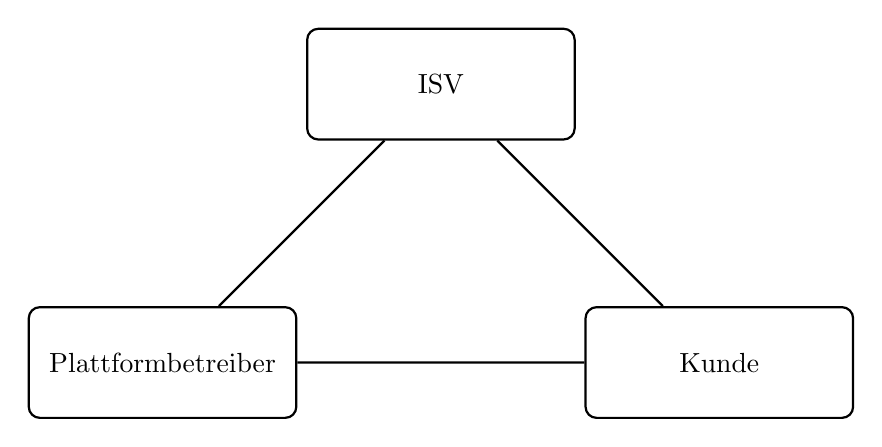
\begin{tikzpicture}[auto]
    \node[b] (ISV) {ISV};
    \node[b,below left of=ISV] (PAAS) {Plattformbetreiber};
    \node[b,below right of=ISV] (CLIENT) {Kunde};
    
    \path[l] (ISV) -- (PAAS) -- (CLIENT) -- (ISV);
    
 
\end{tikzpicture}
}
\caption{Das Beziehungsdreieck aus ISV, Plattformbetreiber und 
Kunde. Angelehnt an die Darstellung für SOAs 
aus \cite{changes_in_requirements_engineering}.}
\label{fig:cloud_oekosystem}
\end{center}
\end{figure}

Wie in Abbildung~\ref{fig:cloud_oekosystem} dargestellt, ist der ISV Teil einer 
Dreiecksbeziehung. Er entwickelt Software für die Plattform des Betreibers und 
veröffentlicht sie gegebenenfalls auf einem Marktplatz der Plattform. 
Beispielhaft dafür seien hier Apples App Store oder AppExchange von Salesforce 
genannt. Die Wahl der passenden Plattform ist essentiell für den 
Unternehmenserfolg, da Funktionsausfälle und Performanzprobleme auf den 
ISV zurückfallen können. Um den passenden Betreiber zu wählen, schlägt 
\citeflow{how_saas_changes_an_isvs_business} vier zu berücksichtigende Aspekte 
vor: Anbietergröße, geografische Lage, Zuverlässigkeit und gesetzliche 
Vorgaben. \\

Der Kontakt zum Kunden hängt vom Markt und insbesondere vom Verkaufspreis ab 
(vgl. Abbildung~\ref{fig:einfluss_des_preises_auf_business}). Am Beispiel des 
App Stores gibt es bei kostenlosen oder sehr günstigen Apps keinen oder kaum 
Kundenkontakt in Form von Anwerbungen, Verkaufsgesprächen, Support oder  
Training. Pauschal gesagt, steigen mit dem Preis die Erwartungen des 
Kunden in Bezug auf Ansprechkeit und Anpassbarkeit der Software. 
\pcite{}{}{how_saas_changes_an_isvs_business}

\begin{figure}[ht]
\begin{center}
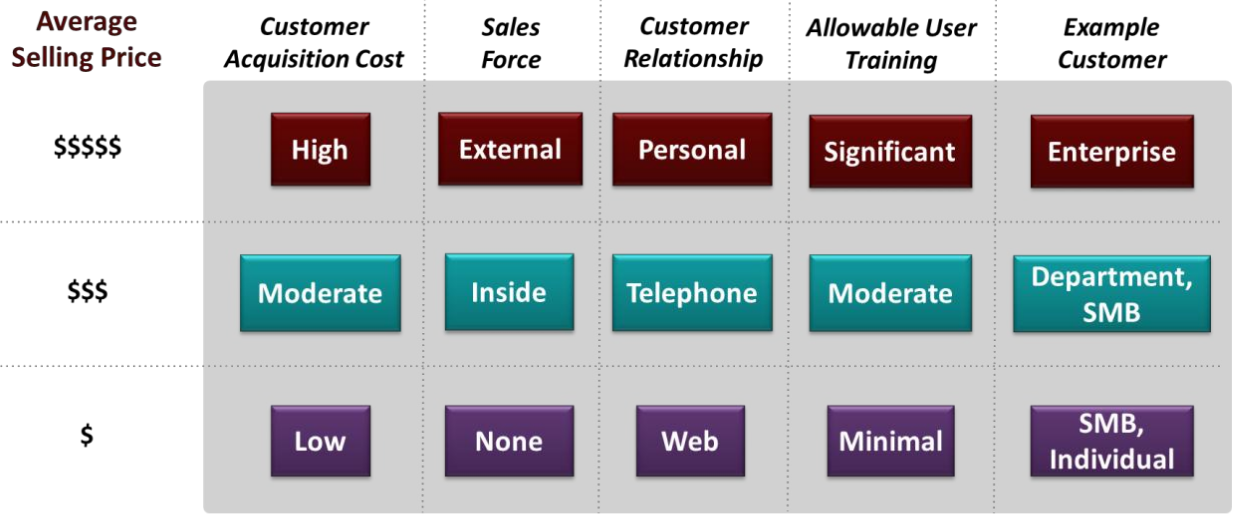
\includegraphics[width=\textwidth]{images/einfluss_des_preises_auf_business.png}
\caption{Der Einfluss des Preises auf das Geschäft. Aus
\protect\citeflow{how_saas_changes_an_isvs_business} }
\label{fig:einfluss_des_preises_auf_business}
\end{center}
\end{figure}

\begin{comment}
\begin{figure}[!h]
\begin{center}
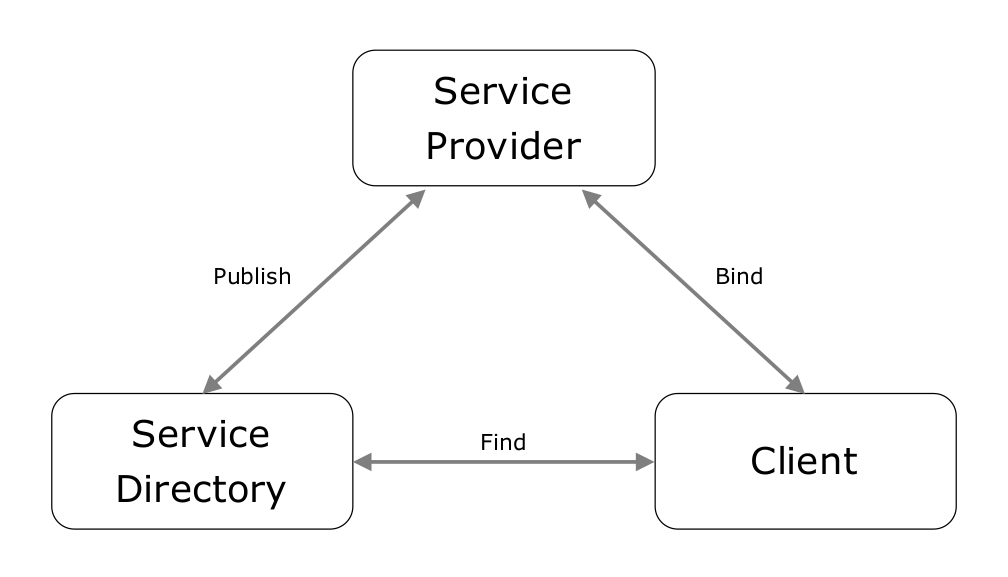
\includegraphics[width=0.8\textwidth]{images/soa_architecture.png}
\caption{Service-oriented architecture. Aus 
\protect\citeflow{changes_in_requirements_engineering}}
\label{fig:soa_architecture}
\end{center}
\end{figure}
\end{comment}

Die Erschließung des Cloud-Marktes wirkt sich auf das Geschäftsmodell des ISV 
aus \pcite{}{}{how_saas_changes_an_isvs_business}:
\begin{description}
	\item[Markt] Das Angebot einer Cloud-Lösung könnte darauf abzielen,
bestehende Kunden und Märkte besser zu erreichen; möglicherweise unter
Kannibalisierung des bestehenden On-Premise-Produktes. Ziel könnte aber auch
sein, neue Märkte zu erschließen. Die beiden Ziele schließen sich nicht aus. Es ist
jedoch wichtig, sich der Möglichkeit der Schwerpunktbildung in dieser Frage
bewusst zu sein.
	\item[Preisgestaltung] Die meisten Preismodelle haben eines der drei 
folgenden Modelle als Grundlage:
	\begin{itemize}
		\item Abonnement -- Zahlung pro Nutzer oder Monat oder pro Gerät und Jahr. Dies
ist das verbreitetste Modell. Durch Vergünstigungen bei Vorauszahlung für einen
längeren Zeitraum, können früh höhere Umsätze generiert werden.
		\item Pro Einheit -- Zahlung für jede Transaktion, jedes
gespeichertes/übertragenes Gigabyte oder für eine andere messbare Einheit, die
einen Nutzungsumfang beschreibt.
		\item Free(mium) -- Das Basisprodukt ist kostenlos nutzbar oder
wird durch Werbeeinblendungen finanziert; Premiumfunktionen müssen bezahlt
werden.
	\end{itemize}
	Die Wahl der Preisgestaltung hat bedeutenden Einfluss auf den Cashflow
des Unternehmens. Gerade die Anfangsinvestition ist bei Cloud-Anwendungen 
häufig größer als bei On-Premise-Anwendungen, gerade wenn das Unternehmen noch 
keine Erfahrungen mit der Umsetzung hat. Diese Anfangsinvestition müssen ISV 
häufig leisten, bevor Kunden akquiriert wurden. \\
Der Einfluss, den die Höhe des Preises auf das Geschäft hat, ist in
Abbildung~\ref{fig:einfluss_des_preises_auf_business} dargestellt. Bei der
Migration in die Cloud sollte darauf geachtet werden, dass der Preis und die
Ausprägungen der anderen Aspekte in der gleichen Zeile liegen.
\begin{comment}
\begin{figure}%[h]
\begin{center}
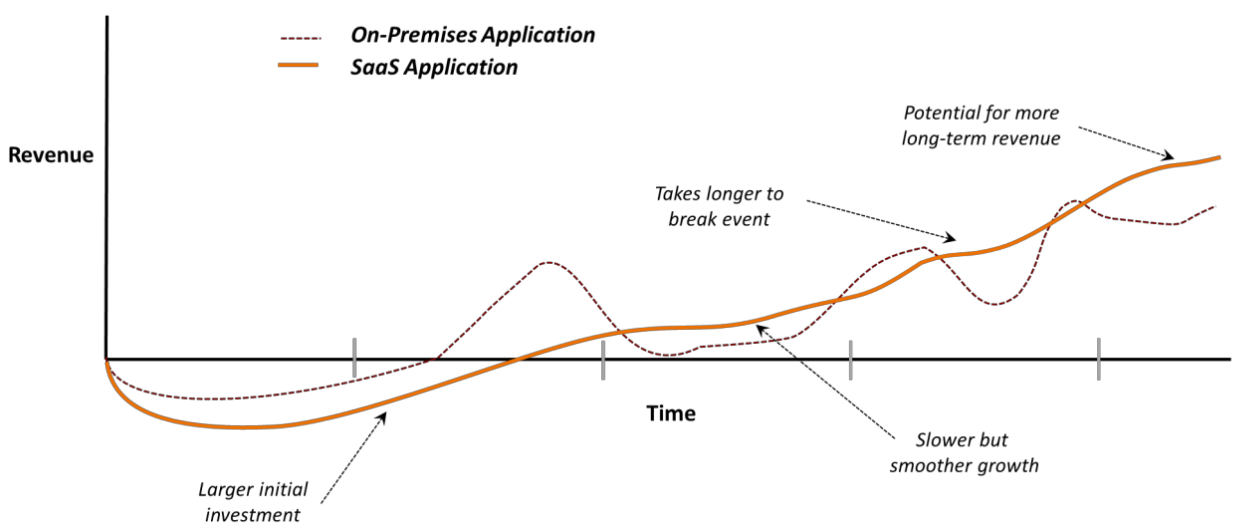
\includegraphics[width=\textwidth]{images/vergleich_umsatz_on-premise_cloud.png}
\caption{Die Umsätze von On-Premise-Anwendungen im Vergleich zu SaaS-
Anwendungen. Aus
\protect\citeflow{how_saas_changes_an_isvs_business} }
\label{fig:vergleich_umsatz_on-premise_cloud}
\end{center}
\end{figure}
\end{comment}
	\item[Verkauf] Bei On-Premise-Anwendungen kann der Kunde die Anwendung
häufig erst nach dem Kauf in seiner Unternehmensumgebung testen und damit den
wahren Produktwert feststellen, weil die Inbetriebnahme für Tests vor dem Kauf zu
aufwändig wäre. Bei Cloud-Anwendungen ist ein ausführliches Testen häufig schon 
vor Abschluss eines großen und langfristigen Lizenzvertrages möglich. Dies ist 
 zunächst ein Vorteil für den Kunden des ISV: Mögliche Fehlinvestitionen lassen 
sich reduzieren oder vermeiden, weshalb Nutzungsentscheidungen des Kunden von 
einer kleineren Gruppe von Managern schneller getroffen werden können. Diese 
reduzierten Einstiegshürden ermöglichen dem ISV eine "`land and 
expand"'-Strategie. Bei der Softwarenutzung bemerkt der Kunde, dass ihm 
Funktionen fehlen oder dass Anpassungen nötig sind, die der ISV im Rahmen von 
Projektverträgen realisieren kann. Für den ISV sinkt das Investitionsrisiko bei der 
Umsetzung von Anforderungen, da er diese nun kennt und nicht mehr vermuten muss. 
Außerdem steigt die Kundenbindung. Zusammenfassend läuft die Entwicklung agiler 
und somit vorteilhafter für den Kunden und den ISV ab.
\end{description}

Die Erschließung der Cloud kann mit drei Organisationsstrukturen erfolgen 
\pcite{}{}{how_saas_changes_an_isvs_business}. Die erste Option besteht darin, 
die Struktur nicht zu verändern, womit der organisatorische Aufwand zunächst 
minimiert wird. Soll das On-Premise-Geschäft jedoch weiter betrieben werden, 
ist es schwierig, in beiden Geschäften wirtschaftlich erfolgreich zu sein, 
wenn Entwickler, die sich eigentlich in 
die neue Technologie einarbeiten sollen, weiterhin an der On-Premise-Software 
arbeiten müssen. Bei Option zwei wird eine Arbeitsgruppe im Unternehmen gebildet, die 
sich ausschließlich mit dem Thema Cloud befasst. Die 
letzte Option besteht darin, diese Gruppe in eine wirtschaftlich selbstständige 
Einheit auszulagern. Mit dieser letzten Option ist der größte organisatorische 
Aufwand verbunden, da mit dem neuen Unternehmen erheblicher Verwaltungsaufwand 
(zum Beispiel Personalmanagement und Buchhaltung) einhergeht.
\begin{comment}
\begin{figure}%[h]
\begin{center}
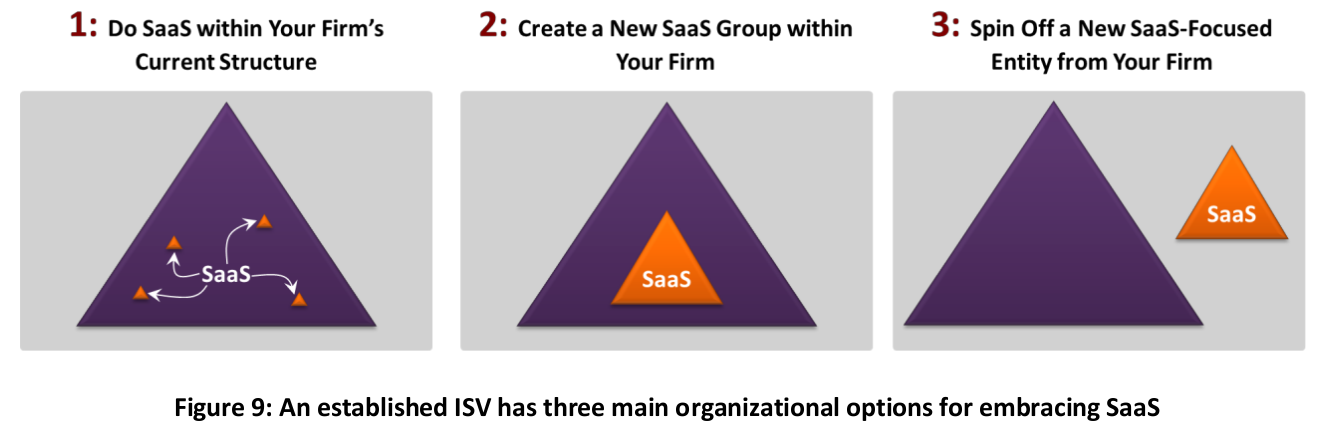
\includegraphics[width=\textwidth]{images/organisationsstrukturen.png}
\caption{Organisationsstrukturelle SaaS-Umsetzungsmöglichkeiten für ISV. Aus
\protect\citeflow{how_saas_changes_an_isvs_business} }
\label{fig:organisationsstrukturen}
\end{center}
\end{figure}

Die Änderungen, die SaaS für das Geschäft bringt überwiegen die
technischen. Da Änderungen aber
sowieso erforderlich sind, um auf
dem Markt zu bestehen, gibt es aber
eigentlich keine Wahl. \pcite{}{}{how_saas_changes_an_isvs_business}
\end{comment}



%\subsection{TODO: Devops als Entwicklungsmodell?}

\begin{comment}
\subsection{Salesforce als Zielplattform}
\label{cha:salesforce_als_zielplattform}
"`Die Ergebnisse belegen: Sämtliche Unternehmen konnten mit Force.com
hinsichtlich Entwicklungszeit und Supportkosten wesentliche Einsparungen
verzeichnen. Die Entwicklung mit Force.com war 4,9-mal schneller als mit JAVA
oder .NET"' \pcite{}{120}{benlian_saas_2010}

Customer Relationship Management (CRM) hat das Ziel Kunden zu gewinnen und zu
halten  und kombiniert dafür die Themen Prozesse, Menschen und Technologie als
übergeordnete Strategie, bei der es darum geht möglichst viel über den Kunden
zu erfahren. Salesforce kommt standardmäßig mit CRM.

Force.com ist eine etablierte Plattform um Cloud-Anwendungen zu entwickeln, zu
vertreiben und bei einer Verfügbarkeit von 99,9\% zu betreiben.
\pcite{}{}{a_new_way_of_developing}
\end{comment}


%\subsection{TODO: Faktoren übernehmen}
%Aus \citeflow{cloud_adoption_decisions}

\subsection{Die Migration bestimmende Faktoren}
\label{cha:migration_bestimmende_faktoren}
\citeflow{fivephases} identifizieren wirtschaftliche und technische Faktoren,
die sowohl die Migrationseignung einer Anwendung als auch die Migration selbst
beeinflussen. \\
\citeflow{decision-making_in_cloud_computing_environments} sehen viele
Parallelen zwischen dem Outsourcen von IT zu externen
Dienstleistern und dem Betrieb in der Cloud, weshalb sich Erfahrungen bei
Outsourcing-Projekten bei Cloud-Migrationen
anwenden lassen. Aus diesem Grund sind die folgenden Faktoren auch aus der
Literatur über IT-Outsourcing zusammengetragen.
\subsubsection{Wirtschaftliche Faktoren}
\begin{description}
	\item[Bereits getätigte IT-Investitionen:]
	In der Regel wachsen die bereits getätigten IT-Ausgaben mit dem
Unternehmen und mit ihnen die Komplexität der Migration. Deshalb ist es in
kleinen Unternehmen eher möglich, direkt zu migrieren, während bei
größeren Unternehmen der Übergang in die Cloud wesentlich mehr Planung und
gegebenenfalls einen parallelen Betrieb erforderlich macht.

	\item[Kosten:] In der herkömmlichen IT bestehen Kosten aus der
"`kapitalintensiven Beschaffung der Hard- und Software, sowie der Vorhaltung
eigener Personalressourcen"' \pcite{}{}{Repschlaeger2010}. Diese Kosten sind
zwar hoch, aber aufgrund der langjährigen Erfahrung auch vorhersagbar und in den 
Budgets eingeplant. Die Migration in die Cloud dagegen bedeutet den Umstieg zu
einem "`pay per use"'-Modell \pcite{}{}{elements_of_cloud_adoption}. Von einem 
Fixkosten-Modell zu einem, das von variablen Kosten bestimmt
ist.
Um zu verhindern, dass Kosteneinsparungen aufgezehrt werden, ist es nötig,
den Umfang der Anwendungsnutzung und die Migrationskosten abzuschätzen und zu 
überwachen.


	\item[Datensicherheit:] Bevor eine Anwendung in die Cloud migriert
wird, sollte bedacht werden, wie kritisch die zugehörigen Daten für den
Unternehmenserfolg und wie sicher sie beim Anbieter sind. Ein Vergleich mit 
Möglichkeiten im Unternehmen ist dabei hilfreich; die Sicherheitskompetenzen 
des Cloud-Anbieters sind häufig größer als die des Unternehmens.
	\item[Rechtliche Restriktionen:] Vor der Migration sollte geprüft
werden, ob rechtliche Bestimmungen auch bei einem Betrieb in der Cloud
eingehalten werden können. Dies kann zum Beispiel bei der Speicherung und 
Verarbeitung personenbezogener Daten relevant sein.
	\item[Zuteilung von Rechenleistungen:] Anwendungen, die kurzzeitig
große Rechenleistungen benötigen und gut skalierbar sein sollen, lassen sich in
der Cloud kostengünstiger betreiben als auf eigenen Servern, die
ganzjährig reserviert sind und die meiste Zeit im Leerlauf verbringen.
\end{description}


\subsubsection{Technische Faktoren}
\begin{description}
	\item[Bestehende Infrastruktur:] Bereits die Migration einer
einzigen Anwendung kann Änderungen in der internen IT-Infrastruktur
erforderlich machen. Zum Beispiel wenn Daten zwischen verschiedenen Diensten
ausgetauscht werden sollen.

	\item[Sicherheitsarchitektur:] Um die Daten im Cloud-Umfeld zu
schützen, muss das bestehende Sicherheitskonzept an die Gegebenheiten der Cloud
angepasst werden.

	\item[Komplexität:]
	Während einfache, standardisierte Anwendungen womöglich bereits in der
Cloud angeboten werden, steigt mit der Komplexität auch der Planungs-,
Implementierungs- und Testaufwand bei der Migration.

	\item[Netzwerk und Support:] Je mehr Daten in der Cloud liegen, desto
höher ist die Abhängigkeit von einer funktionierenden Internetverbindung. Hier
können zusätzliche Kosten für redundante Verbindungen, Verbindungen mit höheren
Kapazitäten oder Verträge mit garantierten Reaktionszeiten im Störungsfall
anfallen.

	\item[IT-Fähigkeiten:] Auch wenn im Cloudbetrieb auf existierende
Technologien und idealerweise existierende Software zurückgegriffen wird,
fordert die Migration dem IT-Team Fähigkeiten und Kenntnisse in den Bereichen
Architekturen, Implementierung, Entwicklung und Betrieb ab. Hinzu kommt, dass
der Umfang, in dem Kontrolle über die Systeme im Cloudbetrieb abgegeben wird,
von den verantwortlichen IT-Mitarbeitern eine "`kulturelle"' Herausforderung
darstellen kann.

	\item[Service Level Agreements (SLAs):] Geprüft werden sollte auch, ob
Cloud-Anbieter SLAs bieten können, die zum unternehmerischen Bedarf
hinsichtlich Verfügbarkeit, Vertraulichkeit und Integrität passen. Auch sollte
geregelt sein, welche Verantwortlichkeiten der Anbieter trägt und welche
Vertragsstrafen bei Nichteinhaltung drohen.
\end{description}


\subsection{Beteiligte Unternehmen und das On-Premise-Produkt iFMS}
\label{cha:replyundifms}

\usetikzlibrary{decorations.text}
\usetikzlibrary{calc}
\usetikzlibrary{fit}
\usetikzlibrary{shapes}
\usetikzlibrary{arrows,positioning} 
\pgfmathsetmacro{\cubex}{4}
\pgfmathsetmacro{\cubey}{2}

\definecolor{light-gray}{gray}{0.80}

\tikzset{
    %Define standard arrow tip
    >=stealth',
    %Define style for boxes
    punkt/.style={
           rectangle,
           rounded corners,
           draw=black, very thick,
           text width=8em,
           minimum height=2em,
           text centered},
    % Define arrow style
    pil/.style={
           ->,
           very thick,
           shorten <=5pt,
           shorten >=5pt,},
    Line/.style={
	dashed,
	very thick
    }
}




%\begin{document}
\begin{figure}[bh]
\begin{center}
\scalebox{1}{
\begin{tikzpicture}

\newcommand{\yOffset}{-1.9*\cubey}
\newcommand{\yOffsetLineBottom}{\yOffset + 0.35*\cubey}
\newcommand{\yOffsetTop}{-0.9*\cubey}
\newcommand{\imgWidthSmall}{0.17\textwidth}
\newcommand{\xOffsetBottom}{0.23*\textwidth}

\coordinate (RO) at (0,0);
\coordinate (LO) at (-\cubex,0);
\coordinate (RU) at (0,-\cubey);
\coordinate (LU) at (-\cubex,-\cubey);
%\draw (RO) -- (RU) -- (LU) -- (LO) -- (RO);
\node[] (reply) at (0,0) 
{
\includegraphics[width=0.45\textwidth]{images/reply.png} };


\node[] (syskoplan) at (0,\yOffset) 
{
\includegraphics[width=\imgWidthSmall]{images/syskoplan.jpg} };
\draw[Line] (0,\yOffsetTop) -- (0,\yOffsetLineBottom);


\node[] (arlanis) at (-\xOffsetBottom,\yOffset) 
{
\includegraphics[width=\imgWidthSmall]{images/arlanis.jpg} };
\draw[Line] (-\xOffsetBottom,\yOffsetTop) -- 
(-\xOffsetBottom,\yOffsetLineBottom);

\node (others) at (\xOffsetBottom,\yOffset) {\Huge{...}};
\draw[Line] (\xOffsetBottom,\yOffsetTop) -- 
(\xOffsetBottom,\yOffsetLineBottom);

\end{tikzpicture}
}
\caption{Das Reply Unternehmensnetzwerk. Eigene Grafik.}
\label{fig:reply}

\end{center}

\end{figure}



Reply ist ein an der italienischen Börse gehandeltes 
IT-Beratungsunternehmen und betrachtet sich als "`Living network"'\ aus 
hochspezialisierten Tochterunternehmen. Seit der Gründung 1996 konnte Reply 
seinen Umsatz auf über 705 Millionen Euro bei 5.245 Angestellten im Jahr 2015 
steigern. Das Netzwerk wuchs und wächst rasch: 2016 wurden bis November drei 
neue Firmen akquiriert. Zwei Tochtergesellschaften, die schon seit mehreren 
Jahren Teil von Reply sind, 
möchte ich genauer vorstellen, da ihre Unternehmensprofile das 
Migrationsprojekt in besonderem Maße beeinflussen.

Die vormalige syskoplan AG, seit dem Erwerb 2010 \pcite{}{12}{replycompprofile} 
Syskoplan Reply, ist ein Spezialist für SAP-Applikationen und 
-Plattformen \pcite{}{10}{replycompprofile} und entwickelt seit 1999 das 
integrierte Facility Management System (iFMS). iFMS verbindet die in SAP 
hinterlegten Daten mit Gebäudeplänen und unterstützt Prozesse rund um die 
Verwaltung von Immobilien. Die gewachsene 
Java-Anwendung mit einer Client-Server-Architektur lässt sich inzwischen nur 
noch schwer warten und um die von Kunden gewünschte Funktionen erweitern. Auch die Bedienung 
über 
eine zusätzlich zu installierenden Anwendung wirkt in Zeiten, in denen Nutzer 
es gewohnt sind, auch umfangreiche Software über den Webbrowser zu bedienen, 
anachronstisch. Beide Aspekte schränken die zukünftige
Wettbewerbsfähigkeit der Software ein. 

Die ehemalige Arlanis Software AG wurde 2012 von Reply übernommen und ist 
Spezialist für Lösungen auf Basis des Cloud Anbieters Salesforce.com. Mit 
Salesforce lassen sich Lösungen häufig ganz ohne eigenen Code auf einer 
SaaS-Basis zusammen klicken. Ist doch Code erforderlich lässt er sich auf der 
PaaS-Plattform (Force.com und Heroku) entwickeln, wobei auf per SaaS angelegte 
Datenmodelle und Daten zugegriffen werden kann, auf die externe Anwendungen per 
Web Service zugreifen können. Mit Salesforce1 steht eine App für mobile Geräte 
zur Verfügung mit der sich jede Salesforce-Anwendung bedienen lässt.

Über das Unternehmensnetzwerk von Reply werden die Stärken beider 
Tochterunternehmen verbunden. Mit dem Know-How im Bereich Facility 
Management und SAP soll auf Salesforce eine innovative, wettbewerbsfähige 
Anwendung geschaffen werden: iFMS@Salesforce.

Die On-Premise-Anwendung iFMS dient dem Facility Management. Mit ihr lassen 
sich Gebäude, Etagen und Räume verwalten, mieten und vermieten. Dabei werden in 
SAP hinterlegte Informationen wie Raumgrößen, Nutzungsarten, Adressen und 
Kontaktinformationen mit CAD Plänen verknüpft. Um iFMS zu nutzen, müssen 
Unternehmen einen Server bereitstellen und instandhalten. Außerdem wird ein Datenbankserver benötigt, auf dem iFMS seine 
Daten speichern kann. Auf dem Rechner eines jeden Nutzers muss ebenfalls eine 
Anwendung installiert werden. 

Ein Screenshot aus Anwendersicht ist in Abbildung~\ref{fig:ifms_liegenschaftsbaum} dargestellt. Sie wird nicht im Detail erklärt, sondern verdeutlicht nur die Art und Komplexität der Anwendung.
\begin{figure}[!h]
\begin{center}
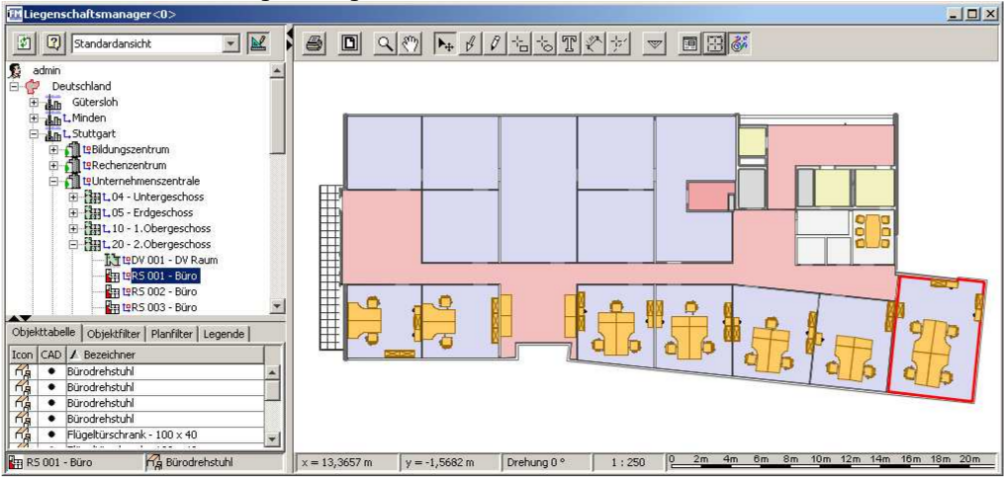
\includegraphics[width=\textwidth]{images/iFMS_liegenschaftsbaum.png}
\caption{Screenshot iFMS aus der 
Benutzerdokumentation (\protect\citeflow{ifms_liegenschaftsmanager}) }
\label{fig:ifms_liegenschaftsbaum}
\end{center}
\end{figure}
Auf der linken Seite lassen sich die Immobilien in einer beliebig 
verzweigbaren Baumstruktur organisieren. So könnten zu den Kategorien in der 
Abbildung "`Land"', "`Stadt"', "`Gebäude"', "`Etagen"' und "`Räume"' zum Beispiel noch "`Kontinente"', 
"`Ländergruppen"', "`Halbetagen"' oder "`Raumteile"' kommen.
Auf der rechten Seite ist der CAD-Plan des Gebäudes bis auf Arbeitsplatzebene 
dargestellt. Arbeitsplätzen können Mitarbeiter, Telefonanschlüsse und beliebige 
Ausrüstungsgegenstände zugeordnet sein. Der Raumplan lässt sich ändern: 
Zwischenwände können gezogen oder entfernt werden. Vertragsdetails, 
Raumnutzungsarten und Bodenbeläge lassen sich - auch für jeden Zeitpunkt in der 
Vergangenheit - visualisieren.

\subsection{Das Fünf-Phasen-Wasserfallmodell}
\label{cha:five_phases}
Das in \citepara{fivephases} vorgeschlagene Vorgehensmodell zur Migration
einer Anwendung in die Cloud ähnelt dem aus der
Softwareentwicklung bekannten, iterativen Wasserfallmodell und besteht aus den
folgenden fünf Phasen, die in Abbildung~\ref{fig:fuenf-phasen-wasserfall-modell}
dargestellt sind. 
\begin{figure}[h]
\begin{center}

\tikzset{
    %Define standard arrow tip
    >=stealth',
    %Define style for boxes
    punkt/.style={
           rectangle,
           rounded corners,
           draw=black, very thick,
           text width=7em,
           minimum height=2em,
           text centered},
    % Define arrow style
    pil/.style={
           ->,
           very thick,
           shorten <=5pt,
           shorten >=5pt,},
    sepLine/.style={
	dashed,
	very thick
    }
}
\scalebox{1.0}{
\begin{tikzpicture}[align=center,node distance=2.2em and 0.6em] 
	\node[punkt] (Machbarkeitsstudie) {Mach\-bar\-keits\-studie} ; 
	\node[punkt] (RE)[below right= of Machbarkeitsstudie]
{An\-for\-der\-ungs\-analyse und Planung};
	\node[punkt] (Migration) [below right= of RE] 
{Migration};
	\node[punkt] (TD) [below right= of Migration] {Test \& De\-ploy\-ment};
	\node[punkt] (Monitoring) [below right= of TD] {Über\-wachung \& 
Wartung};

	\draw[pil] (Machbarkeitsstudie.east) -| (RE.north);
	\draw[pil] (RE.east) -| (Migration.north);
	\draw[pil] (Migration.east) -| (TD.north);
	\draw[pil] (TD.east) -| (Monitoring.north);
	
	\draw[pil] (Monitoring.south) -- ++(0,-5em)coordinate(end);
	\draw[pil] (end) -| (TD.south);
	\draw[pil] (end) -| (Migration.south);
	\draw[pil] (end) -| (RE.south);
	
	
	

\end{tikzpicture}
}
\caption{Das Fünf-Phasen-Wasserfallmodell aus \protect\citeflow{fivephases}}
\label{fig:fuenf-phasen-wasserfall-modell}
\end{center}
\end{figure}

\begin{comment}
\begin{figure}[!h]
\begin{center}
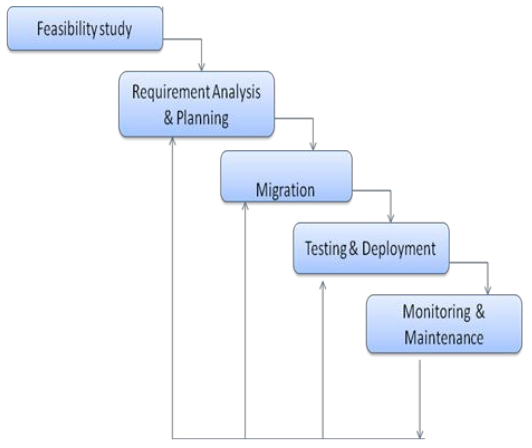
\includegraphics[width=\textwidth]{images/fuenf-phasen-wasserfall-modell.png}
\caption{Das Fünf-Phasen-Wasserfallmodell aus \protect\citeflow{fivephases} }
\label{fuenf-phasen-wasserfall-modell}
\end{center}
\end{figure}
\end{comment}
\begin{description}
	\item[Phase 1 - Machbarkeitsstudie] In dieser Phase wird ergebnisoffen
geprüft, ob die Migration einer Anwendung technisch möglich und wirtschaftlich sinnvoll ist. 
Dabei wird nicht nur die Anwendung selbst analysiert, sondern
auch alle Rahmenbedingungen, die Einfluss auf das Verhalten des Systems ausüben
können. Außerdem wird eine detaillierte Kosten-Nutzen-Analyse erstellt.

	\item[Phase 2 - Anforderungsanalyse und -Planung] Um die zu migrierende
Anwendung und ihre Anforderungen zu verstehen, wird in der Planungsphase die
bestehende IT-Umgebung unter Berücksichtigung der genannten, die Migration
beeinflussenden Faktoren (siehe  Kapitel
\ref{cha:migration_bestimmende_faktoren})
genau begutachtet. Gilt die Anwendung auch nach Begutachtung als zur Migration
geeignet, werden der Return on Investment (ROI) sowie die Total Cost of
Ownership (TCO) berechnet, um die durch die Migration entstehende
Kostenvorteile
zu verstehen.

	\item[Phase 3 - Migration] Die existierende Anwendung wird in die Cloud
portiert und in Hinblick auf Leistungsfähigkeit und Performanz strukturiert
getestet. Zum Schluss wird die neue Plattform in einem User Acceptance Testing
(UAT) validiert.

	\item[Phase 4 - Tests und Auslieferung] Die Daten aus der Produktion
werden in die Cloud portiert. Anschließend wird die Software erneut getestet
und freigegeben. In dieser Phase ist ein hoher Grad an Überwachung und Support
nötig, um unvorhergesehene Probleme auffangen zu können. Unter Umständen wird
parallel zum Start der Cloud-Anwendung die Altsoftware zunächst weiter
betrieben.

	\item[Phase 5 - Überwachung und Wartung] Nach der Migration in die
Cloud ist es naturgemäß notwendig, die Leistungserfüllung durch den Anbieter in
Hinblick auf Leistungsfähigkeit, Verfügbarkeit und Sicherheit zu überwachen um
gegebenenfalls Gegenmaßnahmen einleiten zu können.
\end{description}
Das Fünf-Phasen-Wasserfallmodell, eine Weiterentwicklung des allgemeinen 
Wasserfallmodells, wird in dieser Arbeit als eine dem Leser vermutlich bekannte 
Grundlage genutzt; durch Vergleiche mit diesem lassen sich die Ideen des in dieser Arbeit 
entwickelten Modells einordnen. Dabei stehen die einzelnen Tätigkeiten und 
Aufgaben im Vordergrund, nicht die sequentielle Anordnung, da sie auch Teil 
von agilen Vorgehensweisen ist. 
Unter anderem Namen, aber mit ähnlichem Inhalt, sind die genannten Phasen 
Bestandteile anderer Modelle: 
\citeflow{towards_modelling_a_cloud_applications_life_cycle} beispielsweise 
definieren in ihrem Lebenszyklus für Cloud-Anwendungen die sechs Schritte 
"`Business Case Definition"', "`Decision Phase"', "`Design Phase"', 
"`Test-driven Development Phase"', "`Deployment"' und "`Operations (monitoring, 
updates, resource adaptions, Decommissioning)"'. Ohne genauere Erläuterung 
fallen anhand der Namen Parallelen zu dem Fünf-Phasen-Modell auf.
\begin{comment}
\subsection{Cloud-Computing}
Da die Definition von "`Cloud-Computing"' des National Institute of Standards
and Technology (NIST) \pcite{}{}{NIST} in \citeflow{thoughtsOnCloud} als gute
Grundlage geschätzt wird und auch in \citeflow{fivephases}, in dem das
Fünf-Phasen-Modell vorgestellt wird, als Basis dient, übernehme ich die
Definition in übersetzter Form aus \citeflow{softwareindustrie2015}:
\begin{cloudcomputing}
"`Ein Modell, das einen komfortablen, bedarfsabhängigen und netzbasierten
Zugriff auf eine gemeinsam benutzte Menge konfigurierbarer Rechenressourcen
ermöglicht, die schnell, mit geringem Verwaltungsaufwand und ohne (menschliche)
Interaktion mit einem Anbieter bereitgestellt und wieder freigegeben werden
können."'
\end{cloudcomputing}
Laut NIST besteht die "`Cloud"' als Modell neben fünf Charakteristika und drei
Service Modellen aus vier Einsatzmodellen (im Englischen: "`Deployment
Models"'). Da sie für das Verständnis des Fünf-Phasen-Modells nebensächlich
sind, wird hier nur kurz auf die Einsatzmodelle eingegangen. In ihnen geht es
darum, ob die Cloud ausschließlich von einer Organisation, von einer bestimmten
Gruppe von Organisationen oder von der Öffentlichkeit genutzt wird, wobei auch
Mischformen als Möglichkeit genannt werden. \pcite{}{}{NIST}

\subsubsection{Charakteristika}
Die fünf Charakteristika von Cloud-Computing, die in \citeflow{NIST} genannt
werden, lauten zusammengefasst:

\begin{description}
	\item[Selbstbedienung bei Bedarf:] Ein Nutzer kann ohne
zwischenmenschliche Interaktion mit dem Dienstleister die automatische
Zuteilung von Rechenkapazitäten anstoßen.
	\item[Umfassender Zugriff über das Netzwerk:] Die Dienstleistung ist
über das Netzwerk mit verschiedensten Geräten auf standardisierte Art und Weise
abrufbar, zum Beispiel mit einem Internet Browser.
	\item[Geteilte Ressourcen] Kunden eines Cloud-Anbieters teilen
sich physische oder virtuelle Rechenleistung, die dynamisch und bedarfsgerecht
zugeteilt wird. Im Allgemeinen hat der Nutzer weder Kenntnis noch
Kontrolle über den Ort der Speicherung und Verarbeitung seiner Daten. Abhängig
vom Anbieter lassen sich Orte aber vertraglich festlegen.
	\item[Schnelle Anpassungsfähigkeit] Rechenkapazitäten können dem Bedarf
entsprechend, teilweise automatisch, schnell zugewiesen und entzogen werden.
Auf den Kunden wirkt die abrufbare Rechenleistung oftmals unbegrenzt.
	\item[Vermessene Dienstleistung] Cloud Systeme messen und optimieren
Ressourcennutzung automatisch und stellen die Auslastung und die Nutzung sowohl
dem Cloud Anbieter als auch dem Nutzer zur Verfügung, da sie
Berechnungsgrundlage für die Kosten sind.
\end{description}

\subsubsection{Service Modelle - XaaS}
Service Modelle beschreiben, welche Leistungen "`as a Service"' angeboten
werden. Es gibt recht viele dieser Modelle - \citeflow{xAsAService} zählt 35
Varianten - die mehr oder weniger verbreitet sind und mit "`Everything as a
Service (XaaS)"' zusammengefasst werden. \pcite{}{95}{benlian_saas_2010} Nicht
zwangsläufig beschränkt er sich auf Technologien, die als Dienstleistung
angeboten werden. \pcite{}{872}{decision-making_in_cloud_computing_environments}
\\
\citeflow{NIST} sieht drei Service Modelle vor, die sich im Anteil der
selbst zu verwaltenden, technologischen Anteile (Integrationstiefe)
unterscheiden und in dieser
Hinsicht in Abbildung ~\ref{xaas_im_vergleich} mit der herkömmlichen IT
verglichen werden. Die Wahl des Modells wirkt sich auf den
Migrationsprozess aus. \pcite{}{213}{Pahl2013}
\begin{figure}[hb]
\begin{center}
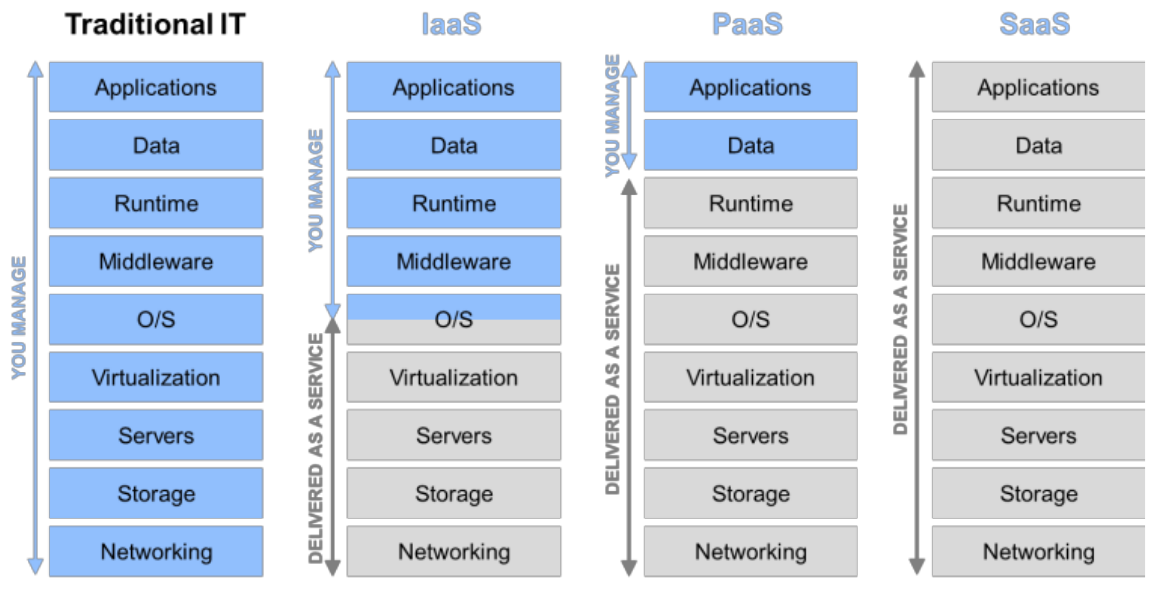
\includegraphics[width=\textwidth]{images/XaaS_im_Vergleich.png}
\caption{XaaS im Vergleich: Umfang von
Dienstleistung und Eigenverantwortung. Aus
\protect\citeflow{economics_of_the_cloud} }
\label{xaas_im_vergleich}
\end{center}
\end{figure}
\begin{description}
	\item[Infrastructure as a Service (IaaS)] Dem Kunden werden Netzwerk,
Speicher und Rechenleistung zur Verfügung gestellt. Über die darauf laufende
Software, teilweise sogar über das Betriebssystem kann selbst verfügt werden. \\
Kunden versprechen sich von IaaS vor allem Flexibilität in der Bereitstellung
und dem Betrieb von Servern, Datenspeichern und Netzwerkressourcen.
\pcite{}{213}{Pahl2013}
	\item[Platform as a Service (PaaS)] Der Kunde kann bereitgestellte
oder selbst entwickelte Software in der Cloud laufen lassen und eventuell
Einfluss auf die Anwendungsumgebung nehmen. \\
	\item[Software as a Service (SaaS)] Der Kunde kann eine vom Anbieter
bereitgestellte Software nutzen und in begrenztem Maße konfigurieren.
\end{description}



\subsecti
Als "`Cloud-Migration"' lässt sich der Begriff als  Diese Bereitstellung in der
Cloud ist zwar unter Umständen
mit keinen oder wenigen Änderungen zu erreichen, sollen aber Vorteile wie
Skalierbarkeit, Kosteneffizienz und Leistung erreicht werden,


Damit ist eine
Cloud-Migration viel mehr als eine Weiterentwicklung.
\pcite{}{}{framework_for_architecture-driven_migration}on{Migrationsformen}


\subsection{Salesforce}

\subsection{Anforderungen eines Independent Software Vendors (ISV)}



\subsection{Ideen}
\begin{description}
	\item[Migration] Sicht eines Unternehmens, das seine
On-Promise-Software in die Cloud schiebt versus ISV
\end{description}


\begin{comment}

\subsection{Herausforderungen in Migrationsprojekten als zu berücksichtigende
Faktoren}
Um die Eignung einer Anwendung für eine Migration in die Cloud zu prüfen,
schlagen \pcite{}{}{fivephases} die Berücksichtigung der folgenden der
folgenden wirtschaftlichen und technischen Faktoren vor. Um diese Faktoren in
einem geordneten Prozess zu berücksichtigen, führen sie ein Vorgehensmodell
ein. Dieses Vorgehensmodell hat den Vorteil, dass es an bestehende Strukturen
und Begrifflichkeiten anknüpft und sich deshalb besonders gut vergleichen,
ergänzen und diskutieren lässt. Aus diesem Grund soll es den Rahmen dieser
Arbeit bilden.

\subsubsection{Wirtschaftliche Faktoren}

\subsubsection{Technische Faktoren}




\subsubsection{Organisationsform als Einflussfaktor}
\citeflow{fivephases} identifizieren die Organisationsstruktur, beziehungsweise
deren Größe und Komplexität und insbesondere drei Formen als
wesentliche Einflussfaktoren für dieses Vorgehensmodell. Zu diesem Ergebnis
kommen auch \citeflow{Pahl2013}.
\begin{description}
	\item[Große Unternehmen] haben gewachsene, komplexe IT-Strukturen, die
umso detailliertere Analysen der Cloud-Eignung einzelner Anwendungen
erforderlich machen und eine Schrittweise Migration nahelegen, bei der
zunächst einfache Standardanwendungen wie E-Mail-Anwendungen migriert werden.
Komplexe Anwendungen folgen sobald Erfahrungen im Cloud-Umfeld gesammelt wurden
und gegebenenfalls fertige Anwendungen in der Cloud bereits existieren.
	\item[Kleinere und mittlere Unternehmen] haben gegenüber großen
Unternehmen nicht nur den Vorteil einer kleineren, weniger komplexen
IT-Landschaft. Bestehende Unternehmensprozesse lassen sich auch leichter an die
Cloud-Nutzung anpassen, sodass sich viele bereits in der Cloud existierende
Cloud-Anwendungen als SaaS nutzen lassen. Durch die nutzungsabhängige
Bepreisung lassen sich in der Cloud möglicherweise Anwendungen nutzen, die
bisher zu teuer oder zu komplex waren. Die nutzungsabhängige Bezahlung birgt
allerdings wie bereits geschildert auch Risiken, die neben den anderen Faktoren
ebenfalls vor der Migrationsentscheidung berücksichtigt werden sollten.
	\item[Regierungsorganisationen] dürften regelmäßig zwei Spezifika
aufweisen, die bei der Prüfung der Cloud-Eignung einer Anwendung zu prüfen
sind. Erstens sind sie in besonderem Maße, teilweise durch Gesetze, zur
Kontrolle über die eigenen Daten und Funktionsfähigkeit ihrer Anwendungen
gezwungen. Zweitens übersteigt die orts-, amts- oder ministerienübergreifende
Zusammenarbeit die Komplexität von großen Unternehmen bei weitem.
\end{description}



\subsection{Methoden zur Anforderungsermittlung in Migrationsprojekten}
\subsection{Aktuelle und prognostizierte Ressourcennutzung}
\subsection{Auswahl des Migrationsziels in der Cloud}
\subsection{Kostenabschätzung der Cloud-Lösung}

\newpage
\subsection{Abbildungen}

\begin{figure}[h]
\begin{center}

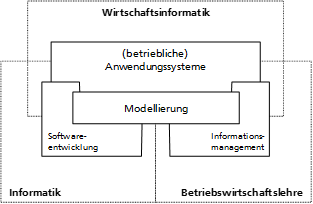
\includegraphics[width=10cm]{images/Abb2_3.png}
\caption{Einordnung der Wirtschaftsinformatik (angelehnt an Fink et al. 2001)}
\label{Abbildung2_3}
\end{center}
\end{figure}
Bitte achten Sie darauf, dass alle vorhandenen Abbildungen und Tabellen in einem inhaltlichen Zusammenhang mit dem Text stehen und Sie auf die entsprechende Abbildung (bspw. Abbildung 1) verweisen.
\subsection{Tabellen}
%hier Tabelle einfügen
\begin{table}[h]
\centering
\begin{tabular}{ccc}
\hline \textbf{Attribute} &\textbf{Typ}  & \textbf{1. Ausprägung (Beispiel)} \\
\hline Titel & \textit{STRING}& Aktiengesetz (AktG)  \\
Text& \textit{STRING} &  [Text des AktG]\\
Gültig von & \textit{DATE} & 01.01.2010 \\
Gültig bis & \textit{DATE} & - \\
Dok.-Besitzer & \textit{STRING} & Rechtsabteilung \\
Quelle & \textit{STRING}  & Deutsche Gesetze \\
Verplichtungsgrad & \textit{STRING} & verplichtend \\
\hline
\end{tabular}
\caption{Attribute der Anforderungsquellen im Metamodell}
\label{tab:tabelle 1}
\end{table}
\par\medskip

Tabelle 1 stellt eine beispielhafte Tabelle dar
\end{comment}
